\chapter{Dataset Profiles Generation and Validation}\label{chapter:roomba}
\graphicspath{{Part1/Chapter2/figures/}}
%%%%%%%%%%%%%%%%%%%%%%%%%
%%%  1. Introduction  %%%
%%%%%%%%%%%%%%%%%%%%%%%%%

\section{Introduction}

The heterogeneous nature of data sources reflects directly on the data quality as they often contain inconsistent as well as misinterpreted and incomplete metadata information. Moreover, the significant variation in size, formats and freshness of the data, makes it more difficult to find useful datasets without prior knowledge. This can be clearly noticed in the LOD Cloud where few datasets such as DBPedia~\cite{Bizer:WebSemJorunal:09}, Freebase~\cite{Bollacker:SIGMOD:08} and YAGO~\cite{Suchanek::WWW:07} are favored over less popular datasets that may include domain specific knowledge more suitable for the tasks at hand. For example, for the task of building context-aware recommender systems in an academic digital library over the LOD cloud, popular datasets like the Semantic Web Dog Food\footnote{\url{http://datahub.io/dataset/semantic-web-dog-food}}, DBLP\footnote{\url{http://datahub.io/dataset/dblp}} or Yovisto\footnote{\url{http://datahub.io/dataset/yovisto}} can be favored over lesser known but more specific datasets like VIAF\footnote{\url{http://datahub.io/dataset/viaf}} which links authority files of 20 national libraries, list of subject headings for public libraries in Spain\footnote{\url{http://datahub.io/dataset/lista-encabezamientos-materia}} or the French dissertation search engine\footnote{\url{http://datahub.io/dataset/thesesfr}}.

Users explore datasets in data portals relying on the metadata information attached by either the dataset owner or the data portal administrator. This information is mainly in form of predefined tags such as \textit{media, geography, life sciences} that are used for organization and clustering purposes. However, the increasing diversity of those datasets makes it harder to classify them in a fixed number of tags that are subjectively assigned without capturing the essence and breadth of the dataset~\cite{Lalithsena:WI:13}. Furthermore, the increasing number of datasets available makes the manual review and curation of metadata unsustainable even when outsourced to communities.

In this chapter, we address the challenges of automatic validation and generation of descriptive datasets profiles. We describe Roomba, an extensible framework consisting of a processing pipeline that combines techniques for data portals identification, datasets crawling and a set of pluggable modules combining several profiling tasks. The framework validates the provided dataset metadata against an aggregated standard set of information. Metadata fields are automatically corrected when possible (e.g., adding a missing license URL reference). Moreover, a report describing all the issues that cannot be automatically fixed is created to be sent by email to the dataset's maintainer. There exist various statistical and topical profiling tools for both relational and Linked Data. The architecture of the framework allows to easily add them as additional profiling tasks. However, in this chapter, we focus on the task of dataset metadata profiling, ignoring the tasks of statistical and topical profiling. We validate our framework against a manually created set of profiles and manually check the accuracy by examining the results of running it on various CKAN-based data portals.

%%%%%%%%%%%%%%%%%%%%%%%
%%%  2. Motivation  %%%
%%%%%%%%%%%%%%%%%%%%%%%

\section{Motivation}

Metadata provisioning is one of the Linked Data publishing best practices mentioned in~\cite{Bizer:DB:11}. Datasets should contain the metadata needed to effectively understand and use them. This information includes the dataset's license, provenance, context, structure and accessibility. The ability to automatically check this metadata helps in:
\begin{itemize}
  \item \textbf{Delaying data entropy}: \textit{Information entropy} refers to the degradation or loss limiting the information content in raw or metadata. As a consequence of information entropy, data complexity and dynamicity, the life span of data can be very short. Even when the raw data is properly maintained, it is often rendered useless when the attached metadata is missing, incomplete or unavailable. Comprehensive high quality metadata can counteract these factors and increase dataset longevity~\cite{Kovacs:GTOS:00}.
  \item \textbf{Enhancing data discovery, exploration and reuse}: Users who are unfamiliar with a dataset require detailed metadata to interpret and analyze accurately unfamiliar datasets. A study conducted by the European Union commission~\cite{Graham:TechReport:11} found that both business and users are facing difficulties in discovering, exploring and reusing public data. due to missing or inconsistent metadata information.
  \item \textbf{Enhancing spam detection}: Portals hosting public open data like Datahub allow anyone to freely publish datasets. Even with security measures like captchas and anti-spam devices, detecting spam is increasingly difficult. In addition to that, the increasing number of datasets hinders the scalability of this process, affecting the correct and efficient spotting of datasets spam.
\end{itemize}

%%%%%%%%%%%%%%%%%%%%%%%%%
%%%  3. Related Work  %%%
%%%%%%%%%%%%%%%%%%%%%%%%%

\section{Related Work}
\label{section:roomba-related-work}
Data Catalog Vocabulary (DCAT)~\cite{Erickson:DCV:14} and the Vocabulary of Interlinked Datasets (VoID)~\cite{Cyganiak:W3C:11} are concerned with metadata about RDF datasets. There exist several tools aiming at exposing dataset metadata using these vocabularies. In~\cite{Bohm:WebSemJournal:11}, the authors generate VoID descriptions limited to a subset of properties that can be automatically deduced from resources within the dataset. However, it still provides data consumers with interesting insights. Flemming's Data Quality Assessment Tool\footnote{\url{http://linkeddata.informatik.hu-berlin.de/LDSrcAss/datenquelle.php}} provides basic metadata assessment as it computes data quality scores based on manual user input. The user assigns weights to the predefined quality metrics and answers a series of questions regarding the dataset. These include, for example, the use of obsolete classes and properties by defining the number of described entities that are assigned disjoint classes, the usage of stable URIs and whether the publisher provides a mailing list for the dataset. The ODI certificate\footnote{\url{https://certificates.theodi.org/}}, on the other hand, provides a description of the published data quality in plain English. It aspires to act as a mark of approval that helps publishers understand how to publish good open data and users how to use it. It gives publishers the ability to provide assurance and support on their data while encouraging further improvements through an ascending scale. ODI comes as an online and free questionnaire for data publishers focusing on certain characteristics about their data. Although these approaches try to perform metadata profiling, they are either incomplete or manual. In our framework, we propose a more automatized and complete approach.

\textbf{Metadata profiling}: The Project Open Data Dashboard\footnote{\url{http://labs.data.gov/dashboard/}} tracks and measures how US government web sites implement the Open Data principles to understand the progress and current status of their public data listings. A validator analyzes machine readable files: e.g., JSON files for automated metrics like the resolved URLs, HTTP status and content-type. However, deep schema information about the metadata is missing like description, license information or tags. Similarly on the LOD cloud, the Datahub LOD Validator\footnote{\url{http://validator.lod-cloud.net/}} gives an overview of Linked Data sources cataloged on the Datahub. It offers a step-by-step validator guidance to check a dataset completeness level for inclusion in the LOD cloud. The results are divided into four different compliance levels from basic to reviewed and included in the LOD cloud. Although it is an excellent tool to monitor LOD compliance, it still lacks the ability to give detailed insights about the completeness of the metadata and overview on the state of the entire LOD cloud group and it is very specific to the LOD cloud group rules and regulations.

\textbf{Statistical profiling}: Calculating statistical information on datasets is vital to applications dealing with query optimization and answering, data cleansing, schema induction and data mining~\cite{Jentzsch:ISWC:14,Frosterus:Springer:11,Lalithsena:WI:13}. Semantic sitemaps~\cite{Cyganiak:ESWC:08} and RDFStats~\cite{Lanegger:DEXA:09} are one of the first to deal with RDF data statistics and summaries. ExpLOD~\cite{Khatchadourian:ESWC:10} creates statistics on the interlinking between datasets based on \texttt{owl:sameAs} links. In~\cite{Li:WISM:12}, the author introduces a tool that induces the actual schema of the data and gathers corresponding statistics accordingly. LODStats ~\cite{Auer:EKAW:12} is a stream-based approach that calculates more general dataset statistics. ProLOD++~\cite{Abedjan:ICDE:14} is a Web-based tool that allows LOD analysis via automatically computed hierarchical clustering~\cite{Bohm:ICDEW:10}. Aether~\cite{Makela:ESWC:14} generates VoID statistical descriptions of RDF datasets. It also provides a Web interface to view and compare VoID descriptions. LODOP~\cite{Forchhammer:PROFILES:14} is a MapReduce framework to compute, optimize and benchmark dataset profiles. The main target for this framework is to optimize the runtime costs for Linked Data profiling. In~\cite{Kaafer:ESWC:13} authors calculate certain statistical information for the purpose of observing the dynamic changes in datasets.

\textbf{Topical Profiling}: Topical and categorical information facilitates dataset search and reuse. Topical profiling focuses on content-wise analysis at the instances and ontological levels. GERBIL~\cite{Usbeck:WWW:15} is a general entity annotation framework that provides machine processable output allowing efficient querying. In addition, there exist several entity annotation tools and frameworks~\cite{Cornolti:WWW:13} but none of those systems are designed specifically for dataset annotation. In~\cite{Frosterus:ESWC:11}, the authors created a semantic portal to manually annotate and publish metadata about both LOD and non-RDF datasets. In~\cite{Lalithsena:WI:13}, the authors automatically assigned Freebase domains to extracted instance labels of some of the LOD Cloud datasets. The goal was to provide automatic domain identification, thus enabling improving datasets clustering and categorization. In~\cite{Bohm:CIKM:12}, the authors extracted dataset topics by exploiting the graph structure and ontological information, thus removing the dependency on textual labels. In ~\cite{Fetahu:ESWC:14}, the authors generate VoID and VoL descriptions via a processing pipeline that extracts dataset topic models ranked on graphical models of selected DBpedia categories.

\textbf{Dataset Search}: Dataset search can be done without relying on attached metadata (tags and categories). For example, there exist several approaches to create LOD indexes. In~\cite{Alexander:LDOW:09}, the authors used VoID descriptions to optimize query processing by determining relevant query-able datasets. In~\cite{Harth:WWW:10}, the authors created an approximate index structure (QTree) and an algorithm for answering conjunctive queries over Linked Data. SchemEX~\cite{Konrath:WebSemJorunal:12} is a stream-based approach leveraging type and property information of RDF instances to create schema-level indexes.

Semantic search engines like Sindice~\cite{Delbru:ESWC:10}, Swoogle~\cite{Ding:CIKM:04} and Watson~\cite{daquin:SemWebJorunal:11} help in entities lookup but they are not designed specifically for dataset search. In~\cite{Nikolov:JIST:11}, the authors utilized the sig.ma index~\cite{Tummarello:WebSemJorunal:10} to identify appropriate data sources for interlinking. Dataset search and discovery is currently done via data portals that rely on attached metadata to provide dataset search features as they run a Solr index on the metadata schemas. Having missing or inconsistent information will affect the search results quality.

Although the above mentioned tools are able to provide various types of information about a dataset, there exists no approach that aggregates this information and is extensible to combine additional profiling tasks. To the best of our knowledge, this is the first effort towards extensible automatic validation and generation of descriptive dataset profiles.

%%%%%%%%%%%%%%%%%%%%%%%%%%%%%%%%%%%
%%%  4. Profiling data portals  %%%
%%%%%%%%%%%%%%%%%%%%%%%%%%%%%%%%%%%

\section{Profiling Data Portals}
\label{section:roomba-framework}
In this section, we provide an overview of Roomba's architecture and the processing steps for validating and generating dataset profiles. Figure \ref{fig:Roomba_architecture} shows the main steps which are the following: (i) data portal identification; (ii) metadata extraction; (iii) instance and resource extraction; (iv) profile validation (v) profile and report generation.

\begin{figure}[!ht]
  \centering
  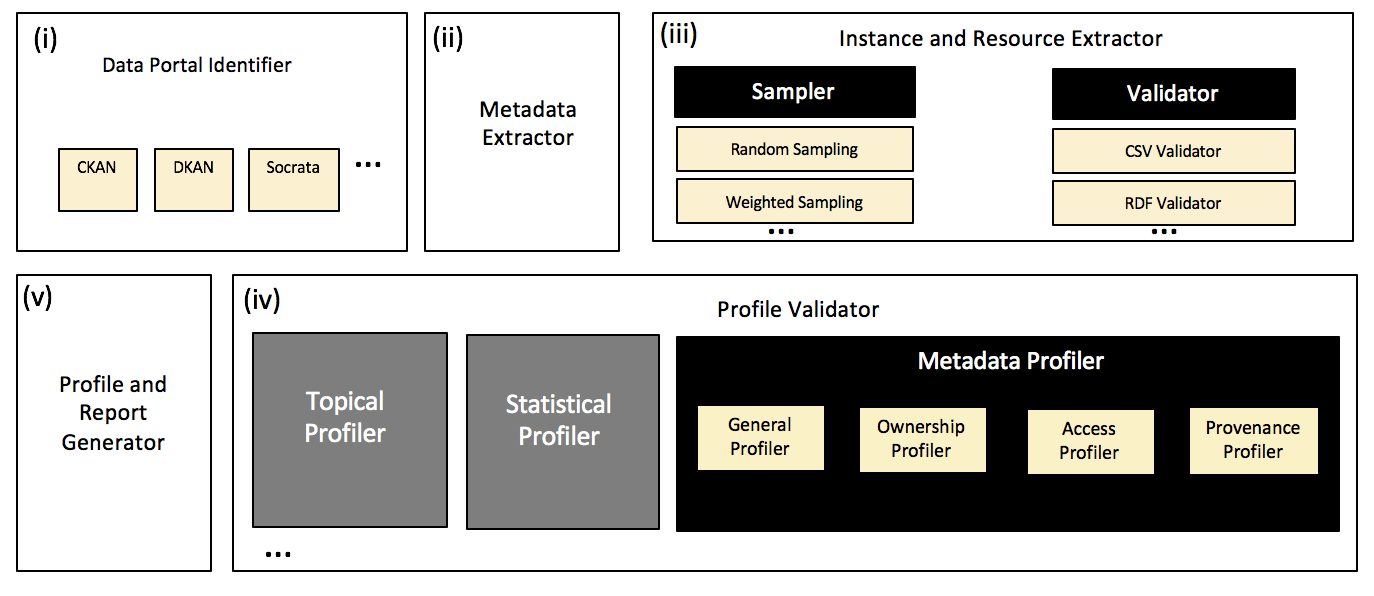
\includegraphics[scale=0.6]{roomba_architecture.png}
  \caption{Processing pipeline for validating and generating dataset profiles}
  \label{fig:Roomba_architecture}
\end{figure}

\pagebreak
Roomba is built as a Command Line Interface (CLI) application (see Figure~\ref{fig:roomba_cli}) using Node.js and is available on the tools Github repository\footnote{\url{https://github.com/ahmadassaf/opendata-checker/tree/master/test}}. Roomba allows data portal administrators like \textbf{Dan} to:

\begin{itemize}
  \item Fetch information about the portal's data management system
	\item Fetch all the information about datasets from a data portal
	\item Fetch all the groups information from a data portal
	\item Crawl, fetch and cache datasets (a specific dataset, datasets in a specific group, 	datasets in the whole portal)
	\item Execute aggregation report on a specific group or on the whole data portal
	\item Profile a specific dataset, a whole group or the whole data portal
\end{itemize}

\begin{figure}[!ht]
  \centering
  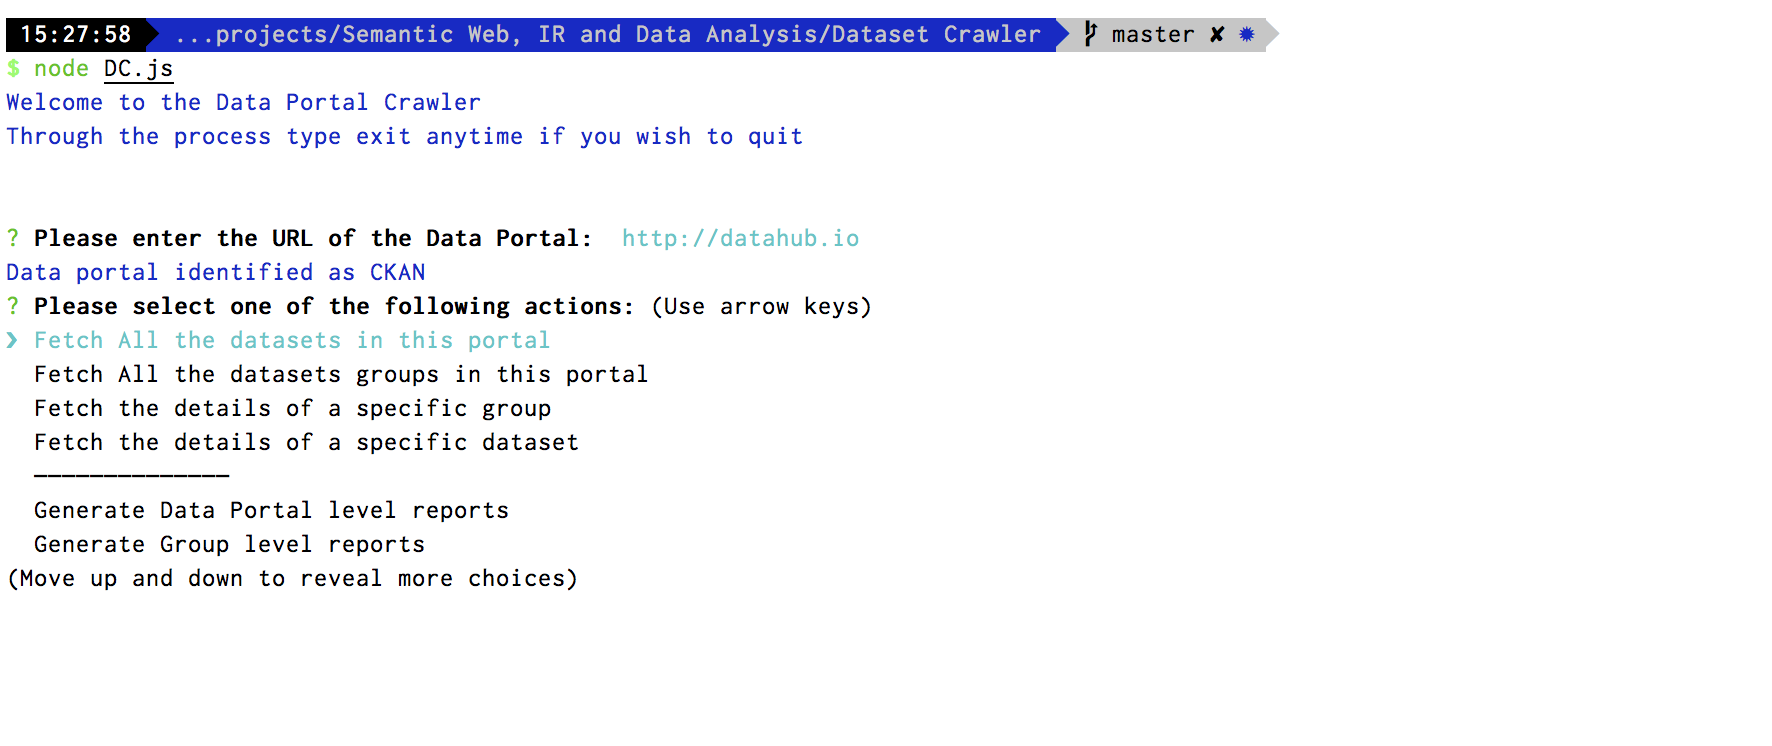
\includegraphics[scale=0.6]{roomba_cli.png}
  \caption{Screenshot for Roomba command line tool}
  \label{fig:roomba_cli}
\end{figure}

Appendix~\ref{section:installation_roomba} details the instructions for installing and running the framework. The various steps are explained in detail below.

\subsection{Data Management System Identification}
Data portals are considered to be data access points providing tools to facilitate data publishing, sharing, searching and visualization. Section~\ref{section:datasetModels} highlights the main data management systems powering those data portals and the various dataset models used. In addition to these traditional data management systems, there is a set of tools that allow exposing data directly as RESTful APIs like Datatank\footnote{\url{http://thedatatank.com}} and Database-to-API\footnote{\url{https://github.com/project-open-data/db-to-api}}.

Roomba is extensible to any data portal. Since every portal has its own API and data model, identifying the software powering data portals is a vital first step. The Data Portal Identifier (component (i)) relies on several Web scraping techniques in the identification process which includes a combination of the following:

\begin{itemize}
  \item \textbf{URL inspection}: Various CKAN based portals are hosted on subdomains of the \texttt{\url{http://ckan.net}}, for example, CKAN Brazil (\texttt{\url{http://br.ckan.net}}). Checking the existence of certain URL patterns can detect such cases.
  \item \textbf{Meta tags inspection}: The \texttt{<meta>} tag provides metadata about the HTML document. They are used to specify page description, keywords, author, etc. Inspecting the \texttt{content} attribute can indicate the type of the data portal. The Data Portal Identifier uses CSS selectors to check the existence of these \texttt{<meta>} tags. An example of a query selector is \texttt{meta[content*=``ckan'']} (all meta tags with the attribute content containing the string $CKAN$). This selector can identify CKAN portals whereas the \texttt{meta[content*=``Drupal'']} can identify DKAN portals.
  \item \textbf{Document Object Model (DOM) inspection}: Similar to the \texttt{<meta>} tags inspection, the Data Portal Identifier checks the existence of certain DOM elements or properties. For example, CKAN-powered portals have DOM elements with class names like \texttt{ckan-icon} or \texttt{ckan-footer-logo}. A CSS selector like \texttt{.ckan-icon} will be able to check if a DOM element with the class name \texttt{ckan-icon} exists.
  The list of elements and properties to inspect is stored in a separate configurable object for each portal. This allows the addition and removal of elements as deemed necessary.
\end{itemize}

The identification process for each portal can be easily customized by overriding the default function. Moreover, adding or removing steps from the identification process can be easily configured.

After those preliminary checks, the Data Portal Identifier issues a query to one of the portal's API endpoints. For example, DataHub is identified as CKAN, so we will query the API endpoint on \texttt{\url{http://datahub.io/api/action/package\_list}}. A successful request will list the names of the site's datasets, whereas a failing request will signal a possible failure of the identification process.

\subsection{Metadata Extraction}
Data portals expose a set of information about each dataset as metadata. The model used varies across portals. However, a standard model (see section~\ref{section:harmonized_metadata}) must contain information about the dataset's title, description, maintainer email, update and creation date, etc.

Since Roomba operates on CKAN-based data portals, the Metadata Extractor (component (ii)) validates the extracted metadata against the CKAN standard model\footnote{\url{http://demo.ckan.org/api/3/action/package\_show?id=adur\_district\_spending}} (see Listing~\ref{ckan_standard_model_excerpt}).

\lstset{basicstyle=\tiny, backgroundcolor=\color{white}, frame=single, caption= {Excerpt of a dataset profile in CKAN standard model}, label=ckan_standard_model_excerpt, captionpos=b}
\lstinputlisting[breaklines=true,language=json]{util/attachments/ckan_model_sample.json}

After identifying the underlying portal software, The Metadata Extractor performs iterative queries to the API in order to fetch datasets metadata and persist them in a file-based cache system. Depending on the portal software, The Metadata Extractor can issue specific extraction jobs. For example, in CKAN-based portals, The Metadata Extractor is able to crawl and extract the metadata of a specific dataset, all the datasets in a specific group (e.g., LOD cloud) or all the datasets in the portal.

\subsection{Instance and Resource Extraction}
From the extracted metadata, the Instance and Resource Extractor (component (iii)) is able to identify all the resources associated with that dataset. They can have various types like a SPARQL endpoint, API, file, visualization, etc. However, before extracting the resource instance(s), the extractor performs the following steps:
\begin{itemize}
  \item \textbf{Resource metadata validation and enrichment}: Check the resource attached metadata values. Similar to the dataset metadata, each resource should include information about its mimetype, name, description, format, valid de-referenceable URL, size, type and provenance. The validation process issues an HTTP request to the resource and automatically fills up various missing information when possible, like the mimetype and size by extracting them from the HTTP response header. However, missing fields like name and description that needs manual input are marked as missing and will appear in the generated summary report.
  \item \textbf{Format validation}: Validate specific resource formats against a linter or a validator. For example, node-csv\footnote{https://github.com/wdavidw/node-csv} for CSV files and n3\footnote{\url{https://github.com/RubenVerborgh/N3.js}} to validate N3 and Turtle RDF serializations.
\end{itemize}

Considering that certain datasets contain large amounts of resources and the limited computation power of some machines on which the framework might run on, a Sampler submodule is introduced to execute various sample-based strategies as they were found to generate accurate results even with comparably small sample size of 10\%~\cite{Fetahu:ESWC:14}. The sampling strategies introduced are:

\begin{itemize}
  \item \textbf{Random Sampling}: Randomly selects resources instances.
  \item \textbf{Weighted Sampling}: Weighs each resource as the ratio of the number of datatype properties used to define a resource over the maximum number of datatype properties over all the datasets resources.
  \item \textbf{Resource Centrality Sampling}: Weighs each resource as the ratio of the number of resource types used to describe a particular resource divided by the total number of resource types in the dataset. This is specific and important to RDF datasets where important concepts tend to be more structured and linked to other concepts.
\end{itemize}

However, the Sampler is not restricted only to these strategies that we offer by default. Strategies like those introduced in~\cite{Leskovec:KDD:06} can be configured and plugged in the processing pipeline.

\subsection{Profile Validation}
A dataset profile should include descriptive information about the data examined. In Roomba, we have identified three main categories of profiling information. However, the extensibility of our framework allows for additional profiling techniques to be plugged in easily (Section ~\ref{section:quality-assessment-framework} describes an extension to measure the objective qualities of datasets).

The Profile Validator (component (iv)) identifies missing information and the ability to automatically correct them. Each set of metadata (general, access, ownership and provenance) is validated and corrected automatically when possible. Each profiler task has a set of metadata fields to check against. The validation process check if each field is defined and if the value assigned is valid.

There exist many special validation steps for various fields. For example, the email addresses and URLs should be validated to ensure that the value entered is syntactically correct. In addition to that, for URLs, the Profile Validator issues an HTTP \texttt{HEAD} request in order to check if that URL is reachable. The Profile Validator also uses the information contained in a valid \texttt{content-header} response to extract, compare and correct some resources metadata values like \texttt{mimetype} and \texttt{size}.

Having valid license information is vital for organization looking to integrate external data. However, from our experiments, we found out that datasets' license information is often missing or noisy. The license names if found are not standardized. For example, \texttt{Creative Commons CCZero} can also be \texttt{CC0} or \texttt{CCZero}. Moreover, the license URI if found and if de-referenceable can point to different reference knowledge bases e.g., \texttt{\url{http://opendefinition.org}}. To overcome this issue, we have manually created a mapping file standardizing the set of possible license names and the reference knowledge base (see Listing~\ref{licenseMappings}). In addition, we have also used the open source and knowledge license information\footnote{\url{https://github.com/okfn/licenses}} to normalize the license information and add extra metadata like the domain, maintainer and open data conformance. The Profile Validator uses this mapping file to valdiate and normalize datasets license information.

\lstset{frame=single, caption={License mapping file sample}, label=json, captionpos=b}
\begin{lstlisting}[language=json]
{
	"license_id" : ["ODC-PDDL-1.0"],
	"disambiguations" : ["Open Data Commons Public Domain Dedication and License (PDDL)"]
},
{
	"license_id" : ["CC-BY-SA-4.0", "CC-BY-SA-3.0"],
	"disambiguations" : ["cc-by-sa", "CC BY-SA","Creative Commons Attribution Share-Alike"]
}
\end{lstlisting}

\subsection{Profile and Report Generation}
The validation process highlights the missing information and presents them in a human readable report (see appendix~\ref{appendix:appendixE}). The report can be automatically sent to the dataset maintainer email if exists in the metadata. In addition to the generated report, the enhanced profiles are represented in JSON using the CKAN data model and are publicly available\footnote{\url{https://github.com/ahmadassaf/opendata-checker/tree/master/results}}.\\

\lstset{basicstyle=\scriptsize, backgroundcolor=\color{white}, breaklines=true, frame=single, caption={Excerpt of the DBpedia validation report}, label=roomba_validation_report, captionpos=b}
\begin{lstlisting}
 =============================================================================
                            Metadata Report
 =============================================================================
  group information is missing. Check organization information as they can be mixed sometimes
  organization_image_url field exists but there is no value defined
 =============================================================================
                            Tag Statistics
 =============================================================================
  There is a total of: 21 [undefined] vocabulary_id fields  100.00%
 =============================================================================
                             License Report
 =============================================================================
  License information has been normalized !
 =============================================================================
                            Resource Statistics
 =============================================================================
  There is a total of: 10 [missing] url-type fields  100.00%
  There is a total of: 9 [missing] created fields  90.00%
  There is a total of: 10 [undefined] cache_last_updated fields  100.00%
  There is a total of: 10 [undefined] size fields  100.00%
  There is a total of: 10 [undefined] hash fields  100.00%
  There is a total of: 10 [undefined] mimetype_inner fields  100.00%
  There is a total of: 7 [undefined] mimetype fields  70.00%
  There is a total of: 10 [undefined] cache_url fields  100.00%
  There is a total of: 6 [undefined] name fields  60.00%
  There is a total of: 9 [undefined] webstore_url fields  90.00%
  There is a total of: 9 [undefined] last_modified fields  90.00%
  There is one [undefined] format field  10.00%
 =============================================================================
                         Resource Connectivity Issues
 =============================================================================
  There are 2 connectivity issues with the following URLs:
    - \url{http://dbpedia.org/void/Dataset}
 =============================================================================
                            Un-Reachable URLs Types
 =============================================================================
 There are: 1 unreachable URLs of type [file]
\end{lstlisting}

Data portal administrators like \textbf{Paul} need an overall knowledge of the portal datasets and their properties. Our framework has the ability to generate numerous reports of all the datasets by passing formatted queries. There are two main sets of aggregation tasks that can be run:
\begin{itemize}
  \item \textbf{Aggregating meta-field values}: Passing a string that corresponds to a valid field in the metadata. The field can be flat like \texttt{license\_title} (aggregates all the license titles used in the portal or in a specific group) or nested like \texttt{resource>resource\_type} (aggregates all the resources types for all the datasets). Such reports are important to have an overview of the possible values used for each metadata field.
  \item \textbf{Aggregating key:object meta-field values}: Passing two meta-field values separated by a colon \texttt{:} e.g., \texttt{resources>resource\_type:resources>name}. These reports are important as you can aggregate the information needed when also having the set of values associated to it printed.
\end{itemize}

For example, the meta-field value query \texttt{resource>resource\_type} run against the LODCloud group will result in an array containing $[file,api,documentation ...]$ values. These are all the resource types used to describe all the datasets of the group. However, to be able to know also what are the datasets containing resources corresponding to each type, we issue a key:object meta-field query\\ \texttt{resource>resource\_type:name}. The result will be a JSON object having the \texttt{resource\_type} as the key and an array of corresponding datasets titles that has a resource of that type.

%%%%%%%%%%%%%%%%%%%%%%%%%%%%%%%%%%%%%%%
%%%  5. Experiments and Evaluation  %%%
%%%%%%%%%%%%%%%%%%%%%%%%%%%%%%%%%%%%%%%

\section{Experiments and Evaluation}
\label{section:roomba_experiment}

In this section, we provide the experiments and evaluation of Roomba. All the experiments are reproducible by our tool and their results are available in its Github repository. A CKAN dataset metadata describes four main sections in addition to the core dataset's properties. These sections are:

\begin{itemize}
  \item \textbf{Resources}: The distributable parts containing the actual raw data. They can come in various formats (JSON, XML, RDF, etc.) and can be downloaded or accessed directly (REST API, SPARQL endpoint).
  \item \textbf{Tags}: Provide descriptive knowledge on the dataset content and structure. They are used mainly to facilitate search and reuse.
  \item \textbf{Groups}: A dataset can belong to one or more group that share common semantics. A group can be seen as a cluster or a curation of datasets based on shared categories or themes.
  \item \textbf{Organizations}: A dataset can belong to one or more organization controlled by a set of users. Organizations are different from groups as they are not constructed by shared semantics or properties, but solely on their association to a specific administration party.
\end{itemize}

Each of these sections contains a set of metadata corresponding to one or more type (general, access, ownership and provenance). For example, a dataset resource will have general information such as the resource name, access information such as the resource url and provenance information such as creation date. The framework generates a report aggregating all the problems in all these sections, fixing field values when possible. Errors can be the result of missing metadata fields, undefined field values or field value errors (e.g., unreachable URL or incorrect email addresses).

\subsection{Experimental Setup}

We ran our tool on two CKAN-based data portals. The first is the Datahub targeting specifically the LOD cloud group. The current state of the LOD cloud report~\cite{Schmachtenberg:ISWC:14} indicates that the LOD cloud contains 1014 datasets. They were harvested via an LDSpider crawler~\cite{Isele:ISWC:10} seeded with 560 thousands URIs. Roomba on the other hand, fetches datasets hosted in data portals where datasets have attached relevant metadata. As a result, we relied on the information provided by the Datahub CKAN API. Examining the tags available, we found two candidate groups. The first tagged with ``lodcloud'' returned 259 datasets, while the second tagged with ``lod'' returned only 75 datasets. After manually examining the two lists, we found out the datasets grouped with the tag ``lodcloud'' are the correct ones as they contained more recent and accurate metadata. To qualify other CKAN-based portals for the experiments, we used \texttt{dataportals.org}, which contains a comprehensive list of Open Data portals from around the world. We chose the Amsterdam data portal \footnote{\url{http://data.amsterdamopendata.nl/}} as it is updated frequently and highly maintained. The portal was commissioned in 2012 by the Amsterdam Economic Board Open Data Exchange (ODE), and covers a wide range of information domains (energy, economy, education, urban development, etc.) about Amsterdam metropolitan region.

The experiments were executed on a 2.6 Ghz Intel Core i7 processor with 16GB of DDR3 memory machine. The approximate execution time alongside the summary of the datasets' properties are presented in table~\ref{table:data_portals_experiments}.

\begin{table}[ht]
\centering
\begin{tabular}{|l|c|c|c|c|}
\hline
Data Portal         & \multicolumn{1}{l|}{No. Datasets} & \multicolumn{1}{l|}{No. Groups} & \multicolumn{1}{l|}{No. Resources} & \multicolumn{1}{l|}{Processing Time} \\ \hline
LOD Cloud           & 259                               & N/A                            & 1068                               & ~140 mins                            \\ \hline
Amsterdam Open Data & 172                               & 18                             & 480                                & ~35 mins                             \\ \hline
\end{tabular}
\caption{Summary of the experiments details}
\label{table:data_portals_experiments}
\end{table}

In our evaluation, we focused on two aspects: i)\textit{profiling correctness} which manually assesses the validity of the errors generated in the report, and ii)\textit{profiling completeness} which assesses if the profilers cover all the errors in the datasets metadata.

\subsection{Profiling Correctness}
To measure profile correctness, we need to make sure that the issues reported by Roomba are valid on the dataset, group and portal levels.

On the dataset level, we choose three datasets from both the LOD Cloud and the Amsterdam data portal. The datasets details are shown in table \ref{table:dataset_experiment}.
\begin{table}[ht]
\centering
\footnotesize\setlength{\tabcolsep}{1.5pt}
\begin{tabular}{|l|c|c|c|c|}
\hline
\textbf{Dataset Name}          & \multicolumn{1}{l|}{\textbf{Data Portal}} & \multicolumn{1}{l|}{\textbf{Group ID}} & \multicolumn{1}{l|}{\textbf{Resources}} & \multicolumn{1}{l|}{\textbf{Tags}} \\ \hline
dbpedia                        & Datahub                                   & lodcloud                               & 10                                      & 21                                 \\ \hline
event-media                    & Datahub                                   & lodcloud                               & 9                                       & 15                                 \\ \hline
bbc-music                      & Datahub                                   & lodcloud                               & 2                                       & 14                                 \\ \hline
bevolking\_cijfers\_amsterdam  & Amsterdam                                 & bevolking                              & 6                                       & 12                                 \\ \hline
bevolking-prognoses-amsterdam  & Amsterdam                                 & bevolking                              & 1                                       & 3                                  \\ \hline
religieuze\_samenkomstlocaties & Amsterdam                                 & bevolking                              & 1                                       & 8                                  \\ \hline
\end{tabular}
\caption{Datasets chosen for the correctness evaluation}
\label{table:dataset_experiment}
\end{table}

To measure the profiling correctness on the groups level, we selected four groups from the Amsterdam data portal containing a total of 25 datasets. The choice was made to cover groups in various domains that contain a moderate number of datasets that can be checked manually (between 3-9 datasets). Table \ref{table:groups_experiment} summarizes the groups chosen for the evaluation.

\begin{table}[ht]
\centering
\begin{tabular}{|l|c|c|c|c|}
\hline
\textbf{Group Name}      & \textbf{Domain}        & \multicolumn{1}{l|}{\textbf{Datasets}} & \multicolumn{1}{l|}{\textbf{Resources}} & \multicolumn{1}{l|}{\textbf{Tags}} \\ \hline
bestuur-en-organisatie   & Management             & 9                                      & 45                                      & 101                                \\ \hline
bevolking                & Population             & 3                                      & 8                                       & 23                                 \\ \hline
geografie                & Geography              & 8                                      & 16                                      & 56                                 \\ \hline
openbare-orde-veiligheid & Public Order \& Safety & 5                                      & 19                                      & 34                                 \\ \hline
\end{tabular}
\caption{Groups chosen for the correctness evaluation}
\label{table:groups_experiment}
\end{table}

After running Roomba and examining the results on the selected datasets and groups, we found out that our framework provides 100\% correct results on the individual dataset level and on the aggregation level over groups. Since our portal level aggregation is extended from the group aggregation, we can infer that the portal level aggregation also produces complete correct profiles. However, the lack of a standard way to create and manage collections of datasets was the source of some errors when comparing the results from these two portals. For example, in Datahub, we noticed that all the datasets \texttt{groups} information were missing, while in the Amsterdam Open Data portal, all the \texttt{organisation} information was missing. Although the error detection is correct, the overlap in the usage of group and organization can give a false indication about the metadata quality.

\subsection{Profiling Completeness}
We analyzed the completeness of our framework by manually constructing a synthetic set of profiles. These profiles cover the range of uncommon problems that can occur in a certain dataset\footnote{\url{https://github.com/ahmadassaf/opendata-checker/tree/master/test}}. These errors are:
\begin{itemize}
 \item Incorrect \texttt{mimetype} or \texttt{size} for resources;
 \item Invalid number of tags or resources defined;
 \item Check if the license information can be normalized via the \texttt{license\_id} or the \texttt{license\_title} as well as the normalization result;
 \item Syntactically invalid \texttt{author\_email} or \texttt{maintainer\_email}.
\end{itemize}

After running our framework at each of these profiles, we measured the completeness and correctness of the results. We found out that our framework covers indeed all the metadata problems that can be found in a CKAN standard model correctly.

%%%%%%%%%%%%%%%%%%%%%%%%%%%%%%%%%%%%%%%
%%%  5. Profiling data portals results  %%%
%%%%%%%%%%%%%%%%%%%%%%%%%%%%%%%%%%%%%%%
\section{Analyzing Profiling Results} \label{section:running_roomba}

In this section, we describe our experiments when running the Roomba tool on the LOD cloud.

Figures \ref{fig:metadata_noise_by_section} and \ref{fig:metadata_noise_by_metadata_type} show the percentage of errors found in metadata fields by section and by information type respectively. We observe that the most erroneous information for the dataset core information is related to ownership since this information is missing or undefined for 41\% of the datasets. Datasets resources have the poorest metadata. 64\% of the general metadata, all the access information and 80\% of the provenance information contain missing or undefined values. Table \ref{table:top_metadata_fields_errors} shows the top metadata fields errors for each metadata information type.

\begin{table}[ht]
\begin{center}
\begin{tabular}{|c|c|c|c|c|c|}
\hline
\multicolumn{2}{|c|}{Metadata Field} & Error \% & Section & Error Type & Auto Fix\tabularnewline
\hline
\hline
\multirow{6}{*}{General } & group & 100\% & Dataset & Missing & -\tabularnewline
\cline{2-6}
 & vocabulary\_id & 100\% & Tag & Undefined & -\tabularnewline
\cline{2-6}
 & url-type & 96.82\% & Resource & Missing & -\tabularnewline
\cline{2-6}
 & mimetype\_inner & 95.88\% & Resource & Undefined & Yes\tabularnewline
\cline{2-6}
 & hash & 95.51\% & Resource & Undefined & Yes\tabularnewline
\cline{2-6}
 & size & 81.55\% & Resource & Undefined & Yes\tabularnewline
\hline
\multirow{5}{*}{Access } & cache\_url & 96.9\% & Resource & Undefined & -\tabularnewline
\cline{2-6}
 & webstore\_url & 91.29\% & Resource & Undefined & -\tabularnewline
\cline{2-6}
 & license\_url & 54.44\% & Dataset & Missing & Yes\tabularnewline
\cline{2-6}
 & url & 30.89\% & Resource & Unreachable & -\tabularnewline
\cline{2-6}
 & license\_title & 16.6\% & Dataset & Undefined & Yes\tabularnewline
\hline
\multirow{5}{*}{Provenance } & cache\_last\_updated & 96.91\% & Resource & Undefined & Yes\tabularnewline
\cline{2-6}
 & webstore\_last\_updated & 95.88\% & Resource & Undefined & Yes\tabularnewline
\cline{2-6}
 & created & 86.8\% & Resource & Missing & Yes\tabularnewline
\cline{2-6}
 & last\_modified & 79.87\% & Resource & Undefined & Yes\tabularnewline
\cline{2-6}
 & version & 60.23\% & Dataset & Undefined & -\tabularnewline
\hline
\multirow{5}{*}{Ownership } & maintainer\_email & 55.21\% & Dataset & Undefined & -\tabularnewline
\cline{2-6}
 & maintainer & 51.35\% & Dataset & Undefined & -\tabularnewline
\cline{2-6}
 & author\_email & 15.06\% & Dataset & Undefined & -\tabularnewline
\cline{2-6}
 & organization\_image\_url & 10.81\% & Dataset & Undefined & -\tabularnewline
\cline{2-6}
 & author & 2.32\% & Dataset & Undefined & -\tabularnewline
\hline
\end{tabular}
\captionof{table}{Top metadata fields error \% by type}
\label{table:top_metadata_fields_errors}
\end{center}
\end{table}

We notice that 42.85\% of the top metadata problems can be fixed automatically. Among them, 44.44\% of these problems can be fixed by our tool while the others need tools that are plugged into the data portal. We further present and discuss the results grouped by metadata information type in the following sub-sections.

\subsection{General Information}
34 datasets (13.13\%) do not have valid \texttt{notes} values. \texttt{tags} information for the datasets are complete except for the \texttt{vocabulary\_id} as this is missing from all the datasets' metadata. All the datasets \texttt{groups} information are missing \texttt{display\_name, description, title, image\_display\_url, id, name}. After manual examination, we observe a clear overlap between group and organization information. Many datasets like \texttt{event-media} use the organization field to show group related information (being in the LOD Cloud) instead of the publishers details.

\subsection{Access Information}
25\% of the datasets access information (being the dataset URL and any URL defined in its groups) have issues: generally missing or unreachable URLs. 3 datasets (1.15\%) do not have a URL defined (tip, uniprot\-databases, uniprot\-citations) while 45 datasets (17.3\%) defined URLs are not accessible at the time of writing this paper. One dataset does not have resources information (bio2rdf\-chebi) while the other datasets have a total of 1068 defined resources.

On the datasets resources level, we notice wrong or inconsistent values in the \texttt{size} and \texttt{mimetype} fields. However, 44 datasets have valid \texttt{size} field values and 54 have valid \texttt{mimetype} field values but they were not reachable, thus providing incorrect information. 15 fields (68\%) of all the other access metadata are missing or have undefined values. Looking closely, we notice that most of these problems can be easily fixed automatically by tools that can be plugged to the data portal. For example, the top six missing fields are the \texttt{cache\_last\_updated}, \texttt{cache\_url}, \texttt{url\-type}, \texttt{webstore\_last\_updated}, \texttt{mimetype\-\_inner} and \texttt{hash} which can be computed and filled automatically. However, the most important missing information which require manual entry are the dataset's \texttt{name} and \texttt{description} which are missing from 817 (76.49\%) and 98 (9.17\%) resources respectively. A total of 334 resources (31.27\%) URLs were not reachable, thus affecting highly the availability of these datasets. CKAN resources can be of various predefined types\\ $(file, file.upload, api, visualization, code, documentation)$. Roomba also breaks down these unreachable resources according to their types: 211 (63.17\%) resources do not have valid \texttt{resource\_type}, 112 (33.53\%) are files, 8 (2.39\%) are metadata and one (0.029\%) is example and documentation types.

To have more details about the resources URL types, we created a $key:object meta-field values$ group level report on the LOD cloud with \texttt{resources>\\format:title}. This aggregates the resources format information for each dataset. We observe that only 161 (62.16\%) of the datasets valid URLs have SPARQL endpoints defined using the \texttt{api/sparql} resource format. 92.27\% provided RDF example links and 56.3\% provided direct links to RDF down-loadable dumps.

The noisiest part of the access metadata is about license information. A total of 43 datasets (16.6\%) does not have a defined \texttt{license\_title} and \texttt{license\_id} fields, where 141 (54.44\%) have missing \texttt{license\_url} field.

\begin{figure}[!ht]
  \centering
  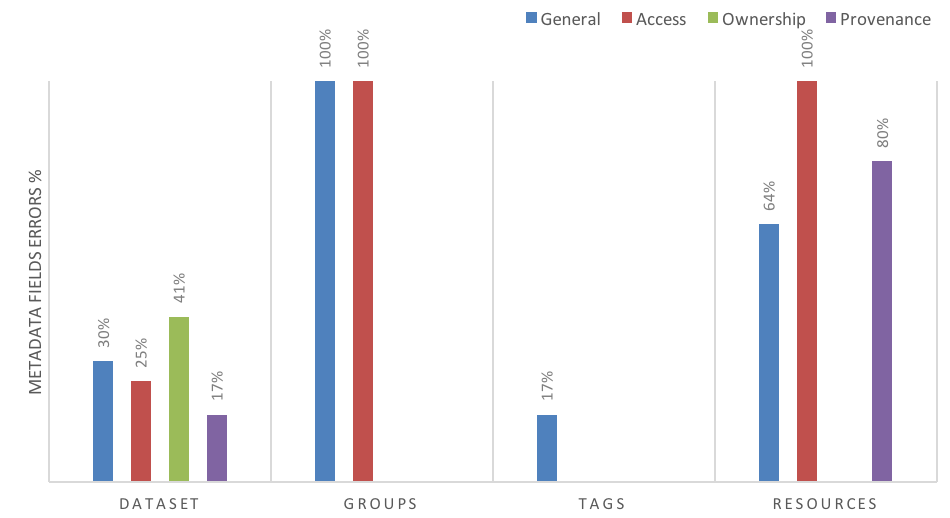
\includegraphics[scale=0.7]{metadata_noise_by_section.png}
  \caption{LOD Cloud error \% by section}
  \label{fig:metadata_noise_by_section}
\end{figure}

\subsection{Ownership Information}
Ownership information is divided into direct ownership (author and maintainer) and organization information. Four fields (66.66\%) of the direct ownership information are missing or undefined. The breakdown for the missing information is: 55.21\% \texttt{maintainer\_email}, 51.35\% \texttt{maintainer}, 15.06\% \texttt{author\_email}, 2.32\% \texttt{author}. Moreover, our framework performs checks to validate existing email values. 11 (0.05\%) and 6 (0.05\%) of the defined \texttt{author\_email} and \texttt{maintainer\_email} fields are not valid email addresses respectively. For the organization information, two field values (16.6\%) were missing or undefined. 1.16\% of the \\\texttt{organization\_description} and 10.81\% of the \texttt{organization\-\_image\_url} information with two out of these URLs are unreachable.

\subsection{Provenance Information}
80\% of the resources provenance information are missing or undefined. However, most of the provenance information (e.g., \texttt{metadata\_created, metadata\_modified}) can be computed automatically by tools plugged into the data portal. The only field requiring manual entry is the \texttt{version} field which was found to be missing in 60.23\% of the datasets.

\subsection{Enriched Profiles}
Roomba can automatically fix, when possible, the license information (title, url and id) as well as the resources mimetype and size.

20 resources (1.87\%) have incorrect \texttt{mimetype} defined, while 52 resources (4.82\%) have incorrect \texttt{size} values. These values have been automatically fixed based on the values defined in the HTTP response header.

We have noticed that most of the issues surrounding license information are related to ambiguous entries. To resolve that, we manually created a mapping file\footnote{\url{https://github.com/ahmadassaf/opendata-checker/blob/master/util/licenseMappings.json}} standardizing the set of possible license names and urls using the open source and knowledge license information\footnote{\url{https://github.com/okfn/licenses}}. As a result, we managed to normalize 123 (47.49\%) of the datasets' license information.

To check the impact of the corrected fields, we seeded Roomba with the enriched profiles. Since Roomba uses file-based cache system, we simply replaced all the datasets \texttt{json} files in the \texttt{\char`\\ cache\char`\\ datahub.io\char`\\ datasets} folder with those generated in \texttt{\char`\\ cache\char`\\ datahub.io\char`\\ enriched}. After running Roomba again on the enriched profiles, we observe that the errors percentage for missing \texttt{size} fields decreased by 32.02\% and for \texttt{mimetype} fields by 50.93\%. We also notice that the error percentage for missing \texttt{license\_urls} decreased by 2.32\%.

\begin{figure}[!ht]
  \centering
  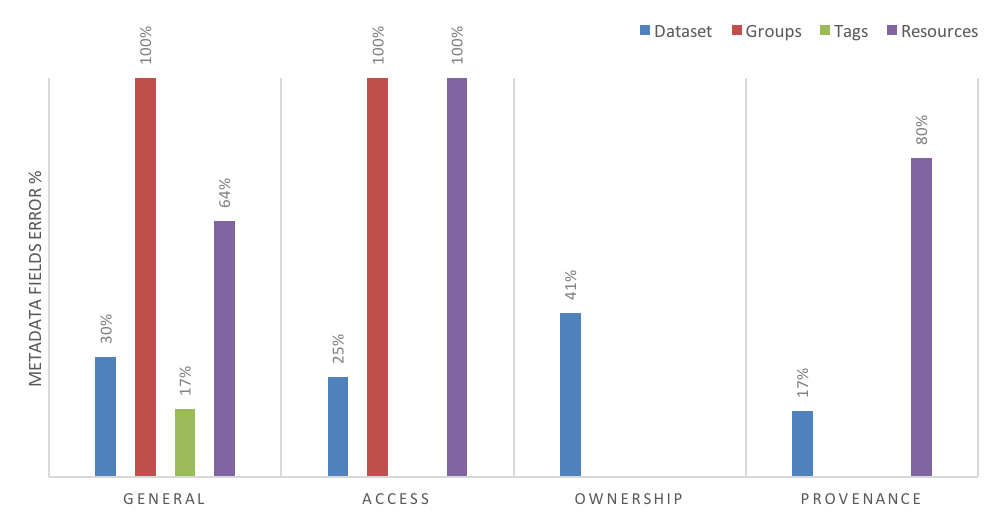
\includegraphics[scale=0.7]{metadata_noise_by_metadata_type.png}
  \caption{LOD Cloud error \% by information type}
  \label{fig:metadata_noise_by_metadata_type}
\end{figure}

\section{Summary}
\label{section:roomba_summary}

In this chapter, we proposed a scalable automatic approach for extracting, validating, correcting and enriching dataset profiles. This approach applies several techniques in order to check the validity of the metadata provided and to generate descriptive and statistical information for a particular dataset or for an entire data portal.

It has been noticed that the issues surrounding metadata quality affect directly dataset search as data portals rely on such information to power their search index. We noted the need for tools that are able to identify various issues in this metadata and correct them automatically. We evaluated our framework manually against two prominent data portals and proved that we can automatically scale the validation of datasets metadata profiles completely and correctly.

We presented the results of running Roomba over the LOD cloud group hosted in the Datahub. We discovered that the general state of the examined datasets needs attention as most of them lack informative access information and their resources suffer low availability. These two metrics are of high importance for enterprises looking to integrate and use external linked data. We found out that the most erroneous information for the dataset core information are ownership related since this information is missing or undefined for 41\% of the datasets. Datasets resources have the poorest metadata: 64\% of the general metadata, all the access information and 80\% of the provenance information contained missing or undefined values. We also showed that the automatic correction process can effectively enhance the quality of some information. We believe there is a need to have a community effort to manually correct missing important information like ownership information (maintainer, author, and maintainer and author emails).

Visiting back our use case scenario, Roomba gives our data portal administrator \textbf{Paul} the ability to discover potential spam datasets by generating flexible report covering the whole range of published datasets. Roomba also ensures that datasets published on his portal contain sufficient attached metadata allowing users like \textbf{Dan} to easily search and discover related datasets.